\documentclass[MASTER.tex]{subfiles}
\begin{document}
	%================================================ %
	\begin{frame}[fragile]
		\frametitle{Negative Binomial Regression with \texttt{R} }
		\Large
		\textbf{Predicted values}
		\begin{itemize}
			\item	For assistance in further understanding the model, we can look at predicted counts for various levels of our predictors. 
			\item Below we create new datasets with values of math and prog and then use the predict command to calculate the predicted number of events.
		\end{itemize}
\end{frame}
	%================================================ %
\begin{frame}[fragile]
		\frametitle{Negative Binomial Regression with \texttt{R} }
		\Large
\begin{itemize}
			\item	First, we can look at predicted counts for each value of prog while holding math at its mean. 
			\item To do this, we create a new dataset with the combinations of prog and math for which we would like to find predicted values, then use the \texttt{predict} command.
		\end{itemize}
	\end{frame}
	%================================================ %
	\begin{frame}[fragile]
		\frametitle{Negative Binomial Regression with \texttt{R} }
		\large
		
		\begin{framed}
			\begin{verbatim}
			
				newdata1 <- data.frame(math = mean(dat$math), 
				prog = factor(1:3, levels = 1:3, 
				labels = levels(dat$prog)))
				
				newdata1$phat <- predict(m1, newdata1, 
				 type = "response")
				 
				newdata1
				    math       prog   phat
				 1 48.27    General 10.237
				 2 48.27   Academic  6.588
				 3 48.27 Vocational  2.850
			
			\end{verbatim}	
		\end{framed}
		
		
	\end{frame}
%================================================ %
\begin{frame}[fragile]
	\frametitle{Negative Binomial Regression with \texttt{R} }
	\Large
	
\begin{itemize}
\item In the output above, we see that the predicted number of events (e.g., days absent) for a general program is about 
10.24, holding math at its mean. 
\item The predicted number of events for an academic program is lower at 6.59, and the predicted number of events for a vocational program is about 2.85.
\end{itemize}
\end{frame}
	%================================================ %
	\begin{frame}[fragile]
		\frametitle{Negative Binomial Regression with \texttt{R} }
		\Large	
	Below we will obtain the mean predicted number of events for values of math across its entire range for each level of prog and graph these.
	\end{frame}

		%================================================ %
		\begin{frame}[fragile]
		\frametitle{Negative Binomial Regression with \texttt{R} }
		\large
		
		\begin{framed}
		\begin{verbatim}
		
			newdata2 <- data.frame(
			math = rep(seq(from = min(dat$math), 
			       to = max(dat$math), length.out = 100), 3),
			prog = factor(rep(1:3, each = 100), levels = 1:3, labels =
			levels(dat$prog)))
		\end{verbatim}	
		\end{framed}
		
		
		\end{frame}
	%================================================ %
	\begin{frame}[fragile]
	\frametitle{Negative Binomial Regression with \texttt{R} }
	\large
	
	\begin{verbatim}
		newdata2 <- cbind(newdata2, predict(m1, newdata2, type = "link", se.fit=TRUE))
		newdata2 <- within(newdata2, {
		DaysAbsent <- exp(fit)
		LL <- exp(fit - 1.96 * se.fit)
		UL <- exp(fit + 1.96 * se.fit)
		})
	\end{verbatim}

\end{frame}

\begin{frame}
\begin{figure}
\centering
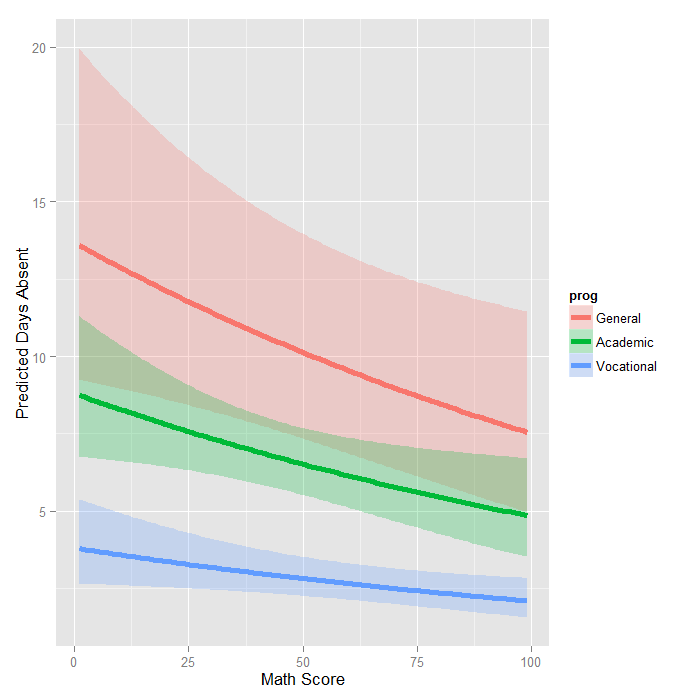
\includegraphics[width=0.7\linewidth]{negbin2}
\caption{}
\label{fig:negbin2}
\end{figure}
	
\end{frame}
	%================================================ %
%	\begin{frame}[fragile]
%		\frametitle{Negative Binomial Regression with \texttt{R} }
%		\large
%		
%		\begin{framed}
%			\begin{verbatim}
%			
%			ggplot(newdata2, aes(math, DaysAbsent)) +
%			geom_ribbon(aes(ymin = LL, ymax = UL, fill = prog), alpha = .25) +
%			geom_line(aes(colour = prog), size = 2) +
%			labs(x = "Math Score", y = "Predicted Days Absent")
%			
%			\end{verbatim}	
%		\end{framed}
%		
%\end{frame}
%================================================ %
\begin{frame}[fragile]
	\frametitle{Negative Binomial Regression with \texttt{R} }
	\Large
	\begin{itemize}
	% Plot of the model predicted days absent with confidence intervals
\item The graph shows the expected count across the range of math scores, for each type of program along with 95 percent confidence intervals. 
\item Note that the lines are not straight because this is a log linear model, and what is plotted are the expected values, not the log of the expected values.
\end{itemize}
\end{frame}


\end{document}